% This must be in the first 5 lines to tell arXiv to use pdfLaTeX, which is strongly recommended.
\pdfoutput=1
% In particular, the hyperref package requires pdfLaTeX in order to break URLs across lines.

\documentclass[11pt]{article}

% Remove the "review" option to generate the final version.
\usepackage{EACL2023}

% Standard package includes
\usepackage{times}
\usepackage{latexsym}
\usepackage{graphicx}

% For proper rendering and hyphenation of words containing Latin characters (including in bib files)
\usepackage[T1]{fontenc}
% For Vietnamese characters
% \usepackage[T5]{fontenc}
% See https://www.latex-project.org/help/documentation/encguide.pdf for other character sets

% This assumes your files are encoded as UTF8
\usepackage[utf8]{inputenc}

% This is not strictly necessary, and may be commented out.
% However, it will improve the layout of the manuscript,
% and will typically save some space.
\usepackage{microtype}

% This is also not strictly necessary, and may be commented out.
% However, it will improve the aesthetics of text in
% the typewriter font.
\usepackage{inconsolata}


% If the title and author information does not fit in the area allocated, uncomment the following
%
%\setlength\titlebox{<dim>}
%
% and set <dim> to something 5cm or larger.

\title{Language Identification from Audio under Severe Speaker Bias\\
 \ NNTI Winter Term Project 2025-26
}


% Author information can be set in various styles:
% For several authors from the same institution:
% \author{Author 1 \and ... \and Author n \\
%         Address line \\ ... \\ Address line}
% if the names do not fit well on one line use
%         Author 1 \\ {\bf Author 2} \\ ... \\ {\bf Author n} \\
% For authors from different institutions:
% \author{Author 1 \\ Address line \\  ... \\ Address line
%         \And  ... \And
%         Author n \\ Address line \\ ... \\ Address line}
% To start a seperate ``row'' of authors use \AND, as in
% \author{Author 1 \\ Address line \\  ... \\ Address line
%         \AND
%         Author 2 \\ Address line \\ ... \\ Address line \And
%         Author 3 \\ Address line \\ ... \\ Address line}

\author{Kashish Mendiratta \\
    7022904 \\
  \texttt{kame00004@stud.uni-saarland.de} \\\And
  Muhammad Saqib \\
  7075880 \\
  \texttt{musa00007@uni-saarland.de} \\}

\begin{document}
\maketitle

\begin{abstract}
We study the identification of spoken languages for 22 Indian languages in a difficult low-resource setting. The dataset is balanced by language labels but each language is represented by only five speakers while training which makes speaker identity an easy shortcut for the model. We first reproduced the provided MMS-300m baseline and inspected its failure modes. We then explored stronger model fine-tuning techniques, freezing strategies and several augmentation schemes aimed at increasing the model performance and reducing speaker overfitting. Our analysis of confusion patterns and per-speaker validation results suggests that the main bottleneck is not class imbalance but poor speaker diversity. Generic augmentation helped only modestly while selective augmentation targeted at the most confused languages worked best in our experiments and reached 43.4\% top-1 accuracy. A broader conclusion is that careful optimization matters but the structure of the dataset itself strongly limits how far performance can improve.
\end{abstract}

\section{Introduction}
At first sight, this task looks like a standard audio classification problem: given a short speech segment, predict one out of 22 Indian languages. In practice, it is much harder. Several languages are related, short utterances do not always contain enough distinctive evidence, and the available training data is limited. The most important constraint, however, is that each language is represented by only five speakers.

This creates a shortcut-learning problem. Instead of learning language-specific acoustic patterns, the model can partly rely on speaker-specific cues such as voice quality, pitch range, or recording style. Because of that, our goal was not only to improve the score but also to understand what the model was actually learning. The work followed the three project tasks: reproduce and improve the baseline, address dataset bias, and analyse the model behaviour.

\section{Dataset and Exploratory Data Analysis}
The dataset contains 22 Indian languages with 400 samples per language and only five speakers per language. In our experiments, the provided training split contained \textbf{8689} samples. The original validation split was further divided into \textbf{1650} validation and \textbf{1650} test examples. Each item includes an audio path, language label, speaker ID, and some additional metadata.

The first result from EDA was that the dataset is roughly balanced by \emph{language}. This means class imbalance is not the main issue. The second, much more important result was that speaker diversity is extremely small. Every language is tied to a tiny set of speakers, which makes it easy for the model to associate a language with a handful of voices.

\begin{figure}[t]
\centering
\includegraphics[width=0.48\columnwidth]{languagedistribution.jpeg}
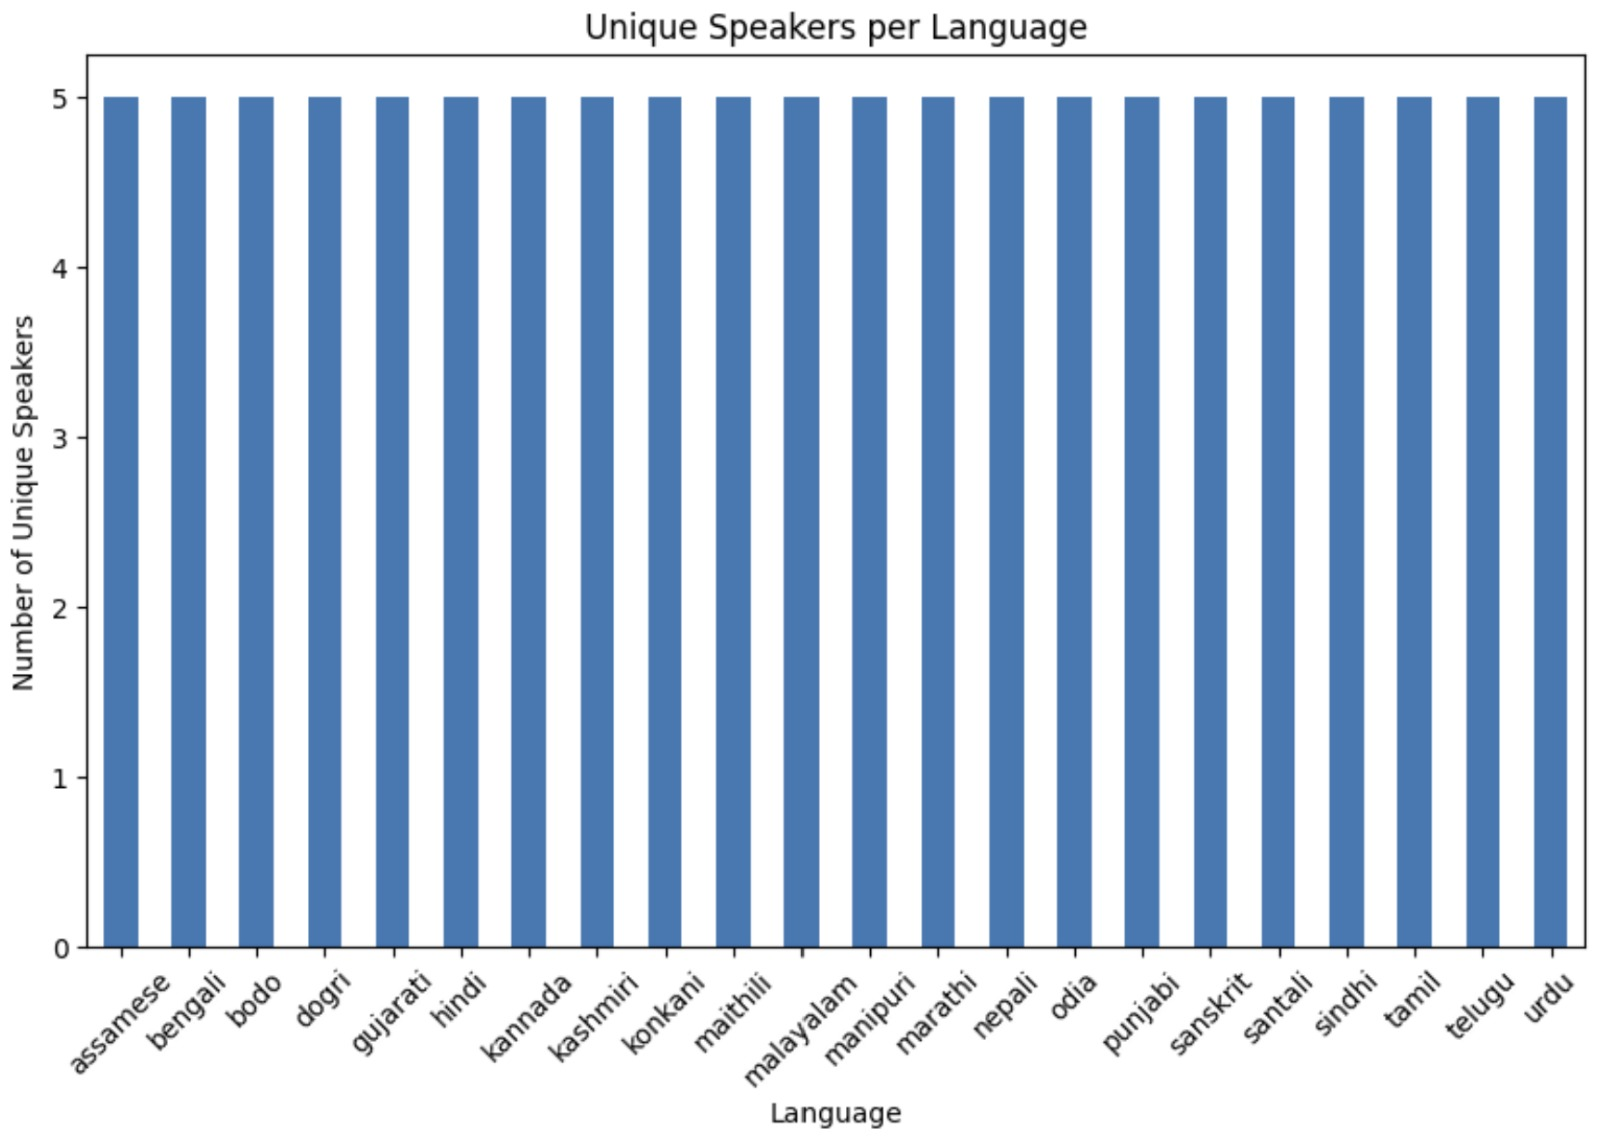
\includegraphics[width=0.48\columnwidth]{Unique_speakers.jpeg}
\caption{EDA summary showing language distribution and number of speakers per language.}
\label{fig:eda}
\end{figure}

\section{Task 1: Reproducing and Improving the Baseline}
We started from the training script provided with the project and tried to reproduce the reported MMS-300m baseline. Simply running the script for three epochs did not reliably reach the result mentioned in the handout. In our runs, training was sensitive to the number of epochs, the learning rate schedule, and how much of the pre-trained model was allowed to update.

The run confirms the main setup of one MMS-based run: learning rate \textbf{$3\times10^{-4}$}, batch size \textbf{128}, \textbf{10} epochs, warmup ratio \textbf{0.1}, and early stopping with patience \textbf{5}. The projector and classifier were reinitialised with small random weights (standard deviation 0.02), which gave a sensible initial loss of \textbf{3.0818}, very close to the random baseline $\log(22)\approx3.09$. The same run had \textbf{75,845,398} trainable parameters out of \textbf{315,706,774} total, or about \textbf{24.02\%}, which means the model was not being fully updated without control.

In the analysed baseline-style run, validation accuracy was \textbf{27.7\%}, with \textbf{1193} wrong predictions out of 1650 samples. The confusion matrix was more informative than the overall score. The model repeatedly confused Hindi with Urdu, Tamil with Malayalam, Telugu with Malayalam, Nepali with Manipuri, and Punjabi with Urdu. Konkani was especially difficult and in one run received an F1-score of \textbf{0.00}. These were not random mistakes; they show that the decision boundary was much weaker for some language groups than for others.

\begin{figure}[t]
\centering
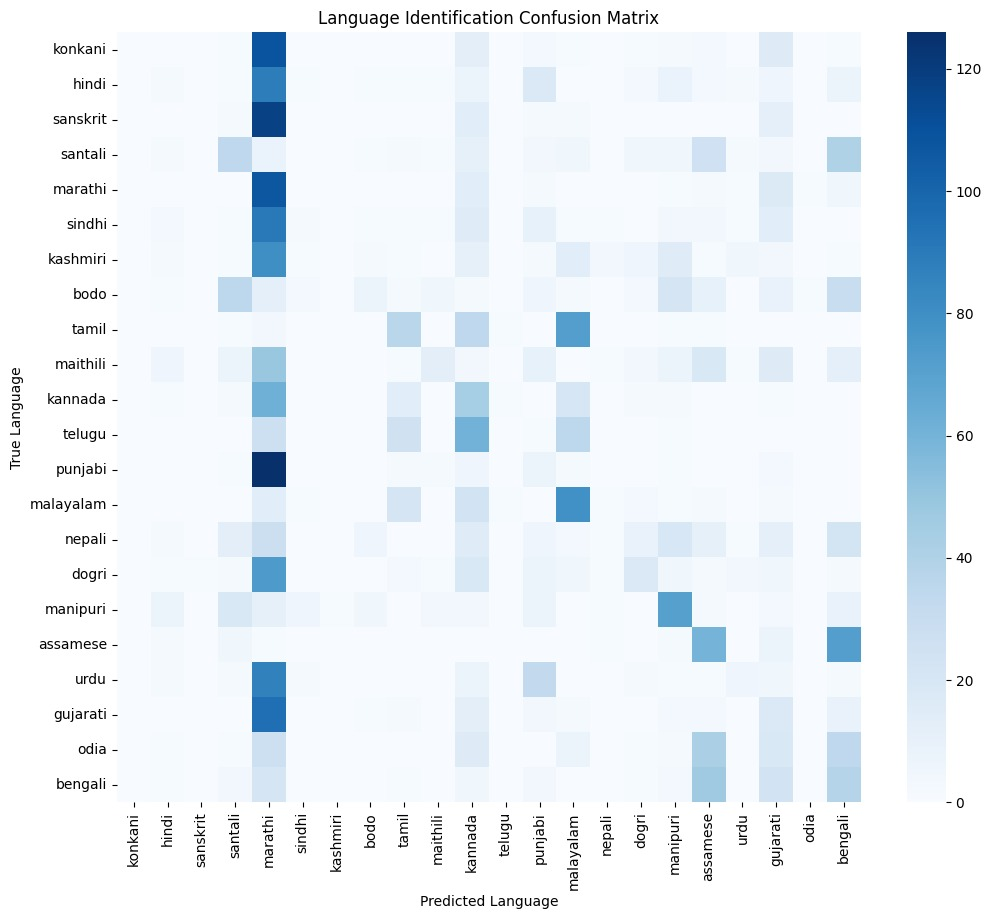
\includegraphics[width=\columnwidth]{Confusion_matrix.jpeg}
\caption{Confusion matrix for the baseline-style MMS system.}
\label{fig:confusions}
\end{figure}

To improve the baseline, we explored three directions: using a different pre-trained model such as XLS-R, tuning optimisation hyperparameters more carefully, and freezing most of the encoder while training only the classification layers. In this low-resource setting, the frozen-encoder setup was usually more stable than aggressive end-to-end fine-tuning, which is consistent with the idea that full fine-tuning can overfit speaker-specific details.

\section{Task 2: Addressing Speaker Bias}
\subsection{How we diagnosed the bias}
The project handout already warned that the model might learn speaker identity instead of language. We wanted to verify that from the results rather than just repeat it. To do that, we evaluated validation performance \emph{per speaker ID inside each language}. For a language $\ell$ and speaker $s$, we computed
\[
\mathrm{Acc}(\ell,s)=\frac{\#\text{correct predictions for speaker }s\text{ in language }\ell}{\#\text{validation samples for speaker }s\text{ in language }\ell}.
\]

A compact way to summarize this is with the within-language standard deviation of speaker-wise accuracy,
\[
\sigma_{\ell}=\mathrm{StdDev}(\{\mathrm{Acc}(\ell,s): s\in S_{\ell}\}).
\]
Large values of $\sigma_{\ell}$ mean the model behaves inconsistently across speakers of the same language. In our analysis, this was one of the clearest signals of speaker bias.

A clear example appeared in Assamese. One speaker ID was classified very well, while others from the same language were much less reliable. Since the language label is the same for all of them, the large spread cannot be explained by language difficulty alone. It suggests that the model had adapted better to some voices than to others.

\begin{table}[t]
\centering
\small
\begin{tabular}{lll}
\toprule
Language & Speaker ID & Validation accuracy / observation \\
\midrule
Assamese & S4258234400382974 & 83\% (very high) \\
Assamese & S4258795500341378 & 12\% \\
Assamese & S4259020500311683 & 89\% (very high) \\
Assamese & S4259066000377409 & 4\% \\
Assamese & S4259615600384226 & 7\%\\
\bottomrule
\end{tabular}
\caption{Illustrative speaker-wise validation behaviour for Assamese showing strong variation between speakers.}
\label{tab:assamese_speakers}
\end{table}
The same kind of spread appeared in other languages as well. This is why we argue that the main bias in the dataset comes from limited speaker diversity. Speakers that are acoustically more similar to the ones the model adapts to tend to perform much better, while others suffer even though they belong to the same class.
\subsection{Augmentation experiments}

To reduce the shortcut based on speaker identity, we experimented with several data-centric and model-based techniques.

\textbf{SpecAugment.} SpecAugment applies time masking and frequency masking to speech features in order to improve model robustness. In our experiments this technique did not improve performance. Although the training loss decreased during optimization, the validation accuracy dropped slightly compared to the baseline. A likely explanation is that aggressive masking removed phonetic cues that are necessary to distinguish languages, especially given the relatively small dataset size.

\textbf{XLS-R model.} We also experimented with the larger multilingual speech model XLS-R. In this setup the encoder was fully fine-tuned and additional regularization techniques such as speed perturbation and dropout were applied. Speed perturbation modifies the speaking rate of audio signals by stretching the waveform (0.9–1.1) and simulates different speaking styles. Despite these improvements, the model achieved lower validation accuracy. The most plausible explanation is that the larger model quickly overfits the limited dataset.

\textbf{Waveform augmentation.} Our augmentation pipeline also included additive noise, gain scaling and speed perturbation applied directly to the waveform before feature extraction. In one run the original training set contained \textbf{8689} examples and \textbf{4344} samples were augmented, increasing the dataset size to \textbf{13033} examples.

We then explored three new strategies: (1) augmentation with replacement, where some originals were replaced by augmented versions; (2) augmentation with sample addition, where original and augmented samples were both kept; and (3) selective augmentation, where extra samples were created mainly for the languages that the baseline confused most often. Generic augmentation gave only modest gains, reaching \textbf{30.85\%} validation accuracy and \textbf{31.58\%} test accuracy in one MMS run. The best result came from the third strategy, \textbf{selective augmentation}, which improved top-1 accuracy to \textbf{43.4\%}. This matched the earlier error analysis: the model benefited more when we targeted the weak decision boundaries instead of perturbing all classes in the same way.

\section{Task 3: Analysis}
The confusion matrix reveals several structured error patterns rather than random mistakes. A strong prediction bias toward certain languages is visible. In particular, many samples from different languages are incorrectly classified as Marathi. This behaviour suggests that the model may have learned speaker-specific acoustic characteristics associated with Marathi speakers rather than language-specific features.

Languages belonging to the Indo-Aryan language family such as Hindi, Urdu, Punjabi, and Gujarati also show significant mutual confusion. These languages share similar phonetic structures and prosodic patterns, which makes them difficult to distinguish using short speech segments. 

In contrast, some languages such as Manipuri and Assamese show stronger diagonal values in the confusion matrix, indicating that the model can identify them more reliably. These languages may contain more distinctive phonetic characteristics that separate them from the other languages in the dataset.

Overall, the confusion matrix highlights two important challenges of the task: acoustic similarity between related languages and the strong speaker bias caused by the limited number of speakers per language.

Language-wise F1 scores further highlight the difficulty of the task. Some languages such as Manipuri, Malayalam and Assamese achieve relatively high F1 scores, indicating that the model can identify them reliably. This behaviour is consistent with the confusion matrix analysis and reflects the acoustic similarity between several languages in the dataset.
\begin{figure}[t]
\centering
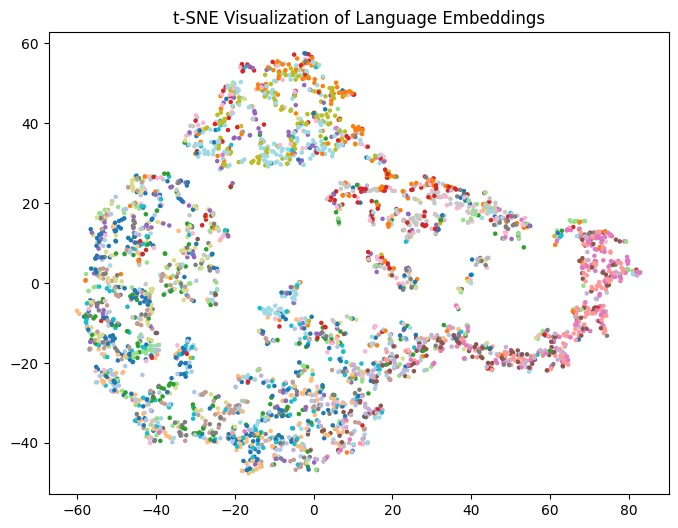
\includegraphics[width=0.8\columnwidth]{t-SNE.jpeg}
\caption{t-SNE visualisation of the last-layer representations. This figure is useful for checking whether the embedding space groups examples more strongly by language or by speaker. Strong speaker-wise clustering would support the speaker-bias argument.}
\label{fig:tsne}
\end{figure}

To inspect the learned representation more directly, we visualised the final-layer embeddings using t-SNE dimensionality reduction. Ideally, samples belonging to the same language would form well-separated clusters in the embedding space.

However, the visualization shows substantial overlap between languages. Instead of forming distinct clusters, many samples from different languages appear intermixed. This suggests that the learned embeddings are not strongly language-specific and that the model captures more general acoustic characteristics.

This observation is consistent with the confusion matrix results, where several languages are frequently misclassified as related languages. One possible explanation is the strong speaker bias in the dataset. Since each language is represented by only five speakers, the model may encode speaker-specific acoustic properties such as pitch, tone or speaking style rather than language identity.

Visualizing the embeddings therefore provides additional evidence that the model has difficulty separating language information from speaker information.

Overall, the project shows that the bottleneck is not just model choice. Even a strong pre-trained model struggles when each language is represented by only a handful of voices. Careful tuning and augmentation help, but they do not completely remove the shortcut.

\section{Conclusion}
In this project we investigated spoken language identification using pretrained speech transform
ers in a challenging low-resource setting. Our baseline MMS model achieved 23.8\% validation
accuracy, which is significantly higher than random chance but still limited by the dataset
constraints.
The improved model achieves a test accuracy of approximately 26.1 percent , which is
significantly higher than the random baseline of 4.54 percent. However, the relatively low
macro F1 score indicates that performance varies substantially across languages.
Experiments with SpecAugment and the larger XLS-R model did not improve performance,
primarily due to the small dataset size and strong speaker bias. Both the confusion matrix
and the t-SNE visualization suggest that the model struggles to learn robust language-specific
representations.
Overall, the results highlight the importance of dataset diversity for speech classification
tasks. Future work could explore more advanced bias mitigation methods such as adversarial
training to explicitly remove speaker information from learned representations.

\section*{References}
\begin{enumerate}

\item PyTorch/Torchaudio. \emph{Audio Data Augmentation Tutorial}.  
\url{https://docs.pytorch.org/audio/stable/tutorials/audio_data_augmentation_tutorial.html}

\item Matthew Baas, Benjamin van Niekerk, and Herman Kamper.  
\emph{Voice Conversion With Just Nearest Neighbors}.  
In \textit{Proceedings of Interspeech}, 2023.

\item Daniel S. Park, William Chan, Yu Zhang, Chung-Cheng Chiu, Barret Zoph, Ekin D. Cubuk, and Quoc V. Le.  
\emph{SpecAugment: A Simple Data Augmentation Method for Automatic Speech Recognition}.  
In \textit{Proceedings of Interspeech}, 2019.

\item Tom Ko, Vijayaditya Peddinti, Daniel Povey, and Sanjeev Khudanpur.  
\emph{Audio Augmentation for Speech Recognition}.  
In \textit{Proceedings of Interspeech}, 2015.

\item Alexei Baevski, Yuhao Zhou, Abdelrahman Mohamed, and Michael Auli.  
\emph{wav2vec 2.0: A Framework for Self-Supervised Learning of Speech Representations}.  
In \textit{Advances in Neural Information Processing Systems (NeurIPS)}, 2020.

\item Arun Babu, Qiantong Wang, Andros Tjandra, and others.  
\emph{XLS-R: Self-Supervised Cross-Lingual Speech Representation Learning at Scale}.  
In \textit{Proceedings of Interspeech}, 2022.

\item Vineel Pratap, Qiantong Xu, Anuroop Sriram, and others.  
\emph{Scaling Speech Technology to 1000+ Languages}.  
\textit{arXiv preprint arXiv:2305.13516}, 2023.

\item Thomas Wolf, Lysandre Debut, Victor Sanh, Julien Chaumond, and others.  
\emph{Transformers: State-of-the-Art Natural Language Processing}.  
In \textit{Proceedings of EMNLP}, 2020.

\item Yaroslav Ganin and Victor Lempitsky.  
\emph{Unsupervised Domain Adaptation by Backpropagation}.  
\textit{arXiv preprint arXiv:1409.7495}, 2014.

\item Yanai Elazar and Yoav Goldberg.  
\emph{Adversarial Removal of Demographic Attributes from Text Data}.  
\textit{arXiv preprint arXiv:1808.06640}, 2018.

\end{enumerate}


\end{document}
